%  TEX program=xelatex

\documentclass[12p,UTF8]{article}
\setlength\paperheight{26cm}
\setlength\paperwidth{18.4cm}
\usepackage[fontset=windows,zihao={-4}]{ctex} % Chinese support, using Windows fonts
\usepackage{setspace} % 导入 setspace 宏包
\usepackage{graphicx} % Insert images
\usepackage{listings} % Print source code
\usepackage{color} % Color support
\usepackage{booktabs} % Professional table support
\usepackage{pdflscape} % Landscape pages support in PDF
\usepackage{hyperref} % Hypertext links support for cross-referencing
\usepackage{geometry} % Page layout customization
\usepackage{float}
\usepackage{subfigure}
\usepackage{fontspec} % 导入 fontspec 宏包，用于设置字体
\setCJKmainfont[BoldFont=SimHei]{SimSun} % 设置中文字体，定义粗体为SimHei
\usepackage{enumitem}
\usepackage{bm} % 在导言区引入 bm 包
\usepackage{ctex}
% \geometry{left = 8 cm, right=8cm , top = 3cm, bottom = 3cm}
% Customize hyperref format (it's set to no special format here)
\hypersetup{hidelinks}
% 设置全局页面边距
\geometry{left=3.17cm, right=3.17cm, top=2.54cm, bottom=2.54cm}
% 设置全局英文字体
\setmainfont{Times New Roman} % 你可以将 Times New Roman 替换为你想要的字体
% Declare directories to search for graphics files for graphicx
\graphicspath{{figures/}{logo/}}



% Define new command for title page
\newcommand{\reporttitle}[2]{
  \LARGE\textsf{#1}\quad\underline{\makebox[12em]{#2}}
}
\newcommand{\reportinfo}[2]{
  \large\makebox[4em]{\textsf{#1}}\quad\underline{\makebox[15em]{#2}}
}

% The document begins here
\begin{document}
\begin{spacing}{1.25} % 设置全局行距为1.25倍
  \begin{titlepage}
     \centering
     % \vspace*{0.2\fill}
     % \vspace*{-20pt}
     \includegraphics[width=\linewidth]{ahu1}\\[3cm] % Change the school logo here (See the logo/ directory) and adjust the height
     % \includegraphics[height=144pt]{pku-text-logo}\\[48pt] % Change the school logo here (See the logo/ directory) and adjust the height
     % {\huge\textsf{课\ 程\ 实\ 验\ 报\ 告}}\\[48pt]
     {\zihao{2} \heiti《数字电路与逻辑设计》\ 综\ 合\ 作\ 业}\\[4cm]
     % \reporttitle{实验名称}{立扫帚实验}\\[72pt]
     % \reportinfo{课程名称}{麻瓜研究}\\[8pt]
     \reportinfo{\zihao{-2}\songti 学\hspace{\fill}院}{\zihao{-2}\songti 电子信息工程学院}\\[10pt]
     \reportinfo{\zihao{-2}\songti 专\hspace{\fill}业}{\zihao{-2}\songti 电子信息工程专业}\\[8pt]
     \reportinfo{\zihao{-2}\songti 年\hspace{\fill}级}{\zihao{-2} \songti 23级}\\[8pt]
     \reportinfo{\zihao{-2}\songti 学\hspace{\fill}号}{\zihao{-2}\songti P12314122}\\[8pt]
     \reportinfo{\zihao{-2}\songti 姓\hspace{\fill}名}{\zihao{-2}\songti 邱云}\\
     \vspace*{\fill}
  \end{titlepage}
  % \newgeometry{left = 3.17cm, right = 3.17cm, top = 2.54cm , bottom=2.54cm}
  \tableofcontents
  \newpage
 \songti
  \section{问题描述与设计要求}
  \subsection{题目描述}
  设计一个基本数字时钟，要求：显示时分秒，显示采用24小时的显示方式。
  % \begin{enumerate}
  %   \item 学会寻找扫帚的重心，培养学生的耐心；
  %   \item 验证基本物理定律在霍格沃茨的有效性。
  % \end{enumerate}
  \subsection{设计要求}
  \begin{enumerate}
    \item 设计一个基本数字时钟；
    \item 可以调节时分秒的数值；
    \item 使用数码管显示时分秒；
    \item 用单个数码管分别显示时，分，秒；
  \end{enumerate}
  \newpage
  \section{设计方案}
  \subsection{总体设计方案}
  数字电子钟有下几部分组成：校正电路、60进制的秒、分计时器和24进制计时计数器以及秒、分、时的译码显示部分等。

  计数结果经过“时”、“分”、“秒”，译码器，显示器显示时间。其中振荡器和分频器组成标准秒脉冲信号发生器，由不同进制的计数器，
  译码器和显示电路组成计时系统。秒信号送入计数器进行计数，把累计的结果以“时”，“分”、“秒”的数字显示出来。“时”显示由十二进制进制计数器，译码器，显示器构成
  ；“分”、“秒”显示分别由六十进制的计数器，译码器，显示器构成；校时电路实现对时，分的校准。
  \begin{figure}[htbp]
    \centering
    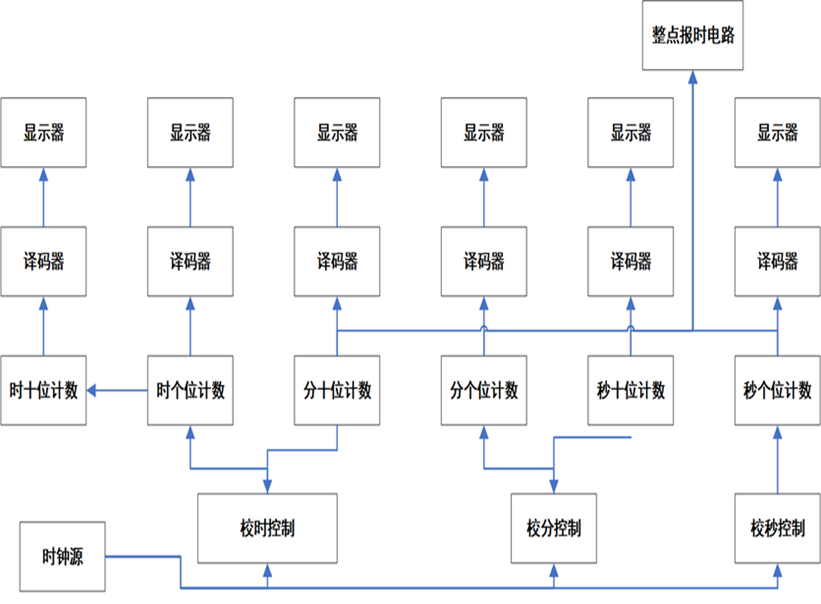
\includegraphics[width=1\textwidth]{alldesign}
    \caption{总设计原理框图}
    \label{alldesign}
  \end{figure}
  \subsubsection{元件选择}

\begin{enumerate}[itemindent=1em]
  \item 主要芯片;
  \begin{itemize}
    \item 74LS160N（4位二进制同步计数器）
    \item 4511BP（七段数码管驱动译码器）
    \item 7408N（与门）
    \item 7404N（非门）
  \end{itemize}
  \item 显示元件;
  \begin{itemize}
    \item 共阴极七段数码管
  \end{itemize}
  \item 其他元器件;
  \begin{itemize}
    \item 电阻、电容、跳线
    \item 开关按键（用于手动复位或调整时间））
    \item 直流稳压电源（5V）
  \end{itemize}
\end{enumerate}
\subsubsection{仿真电路}
总电路仿真图如下图所示：

\begin{figure}[H]
  \centering  %图片全局居中
    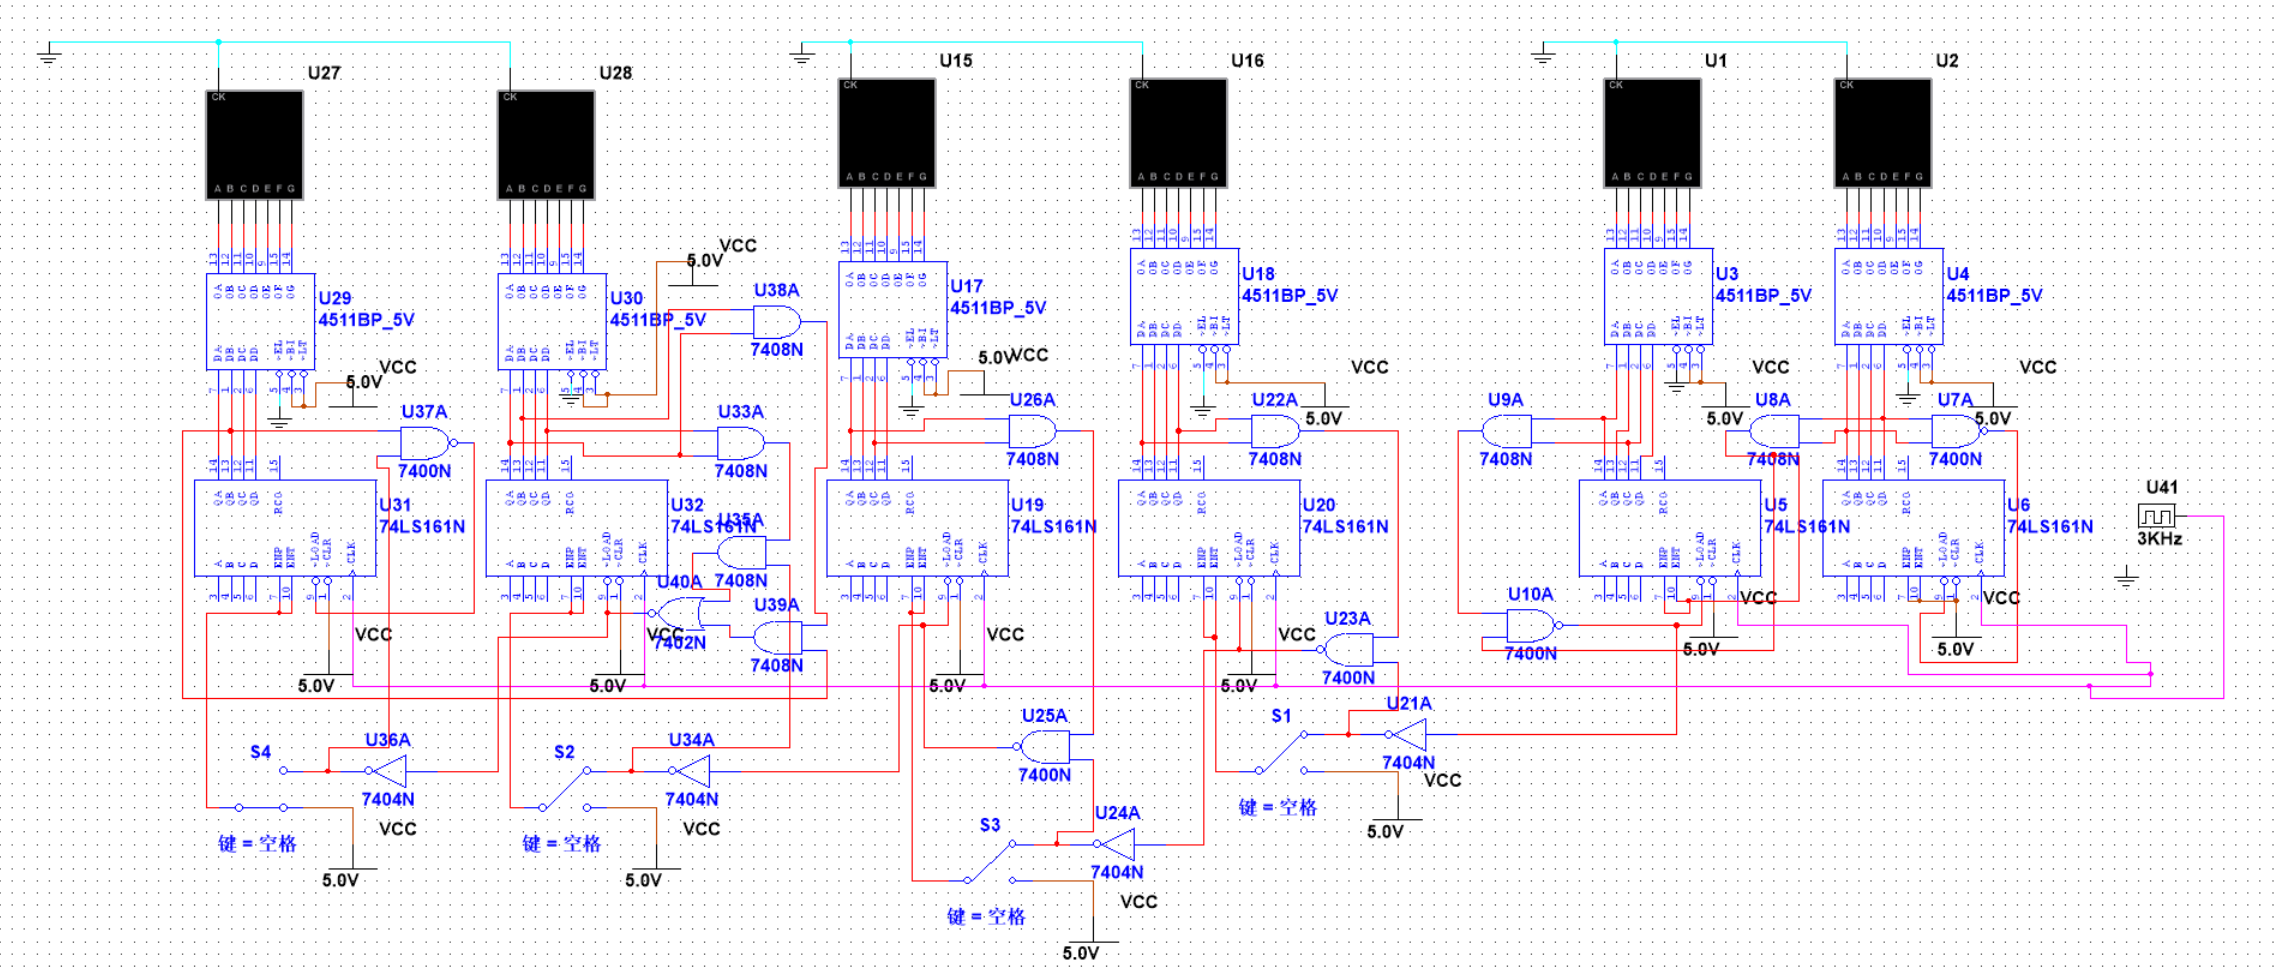
\includegraphics[width=0.9\textwidth]{2p1.png}
    \caption{74LS161仿真}
    \label{2p1}
  \end{figure}
  \begin{figure}[H]
    \centering  %图片全局居中
      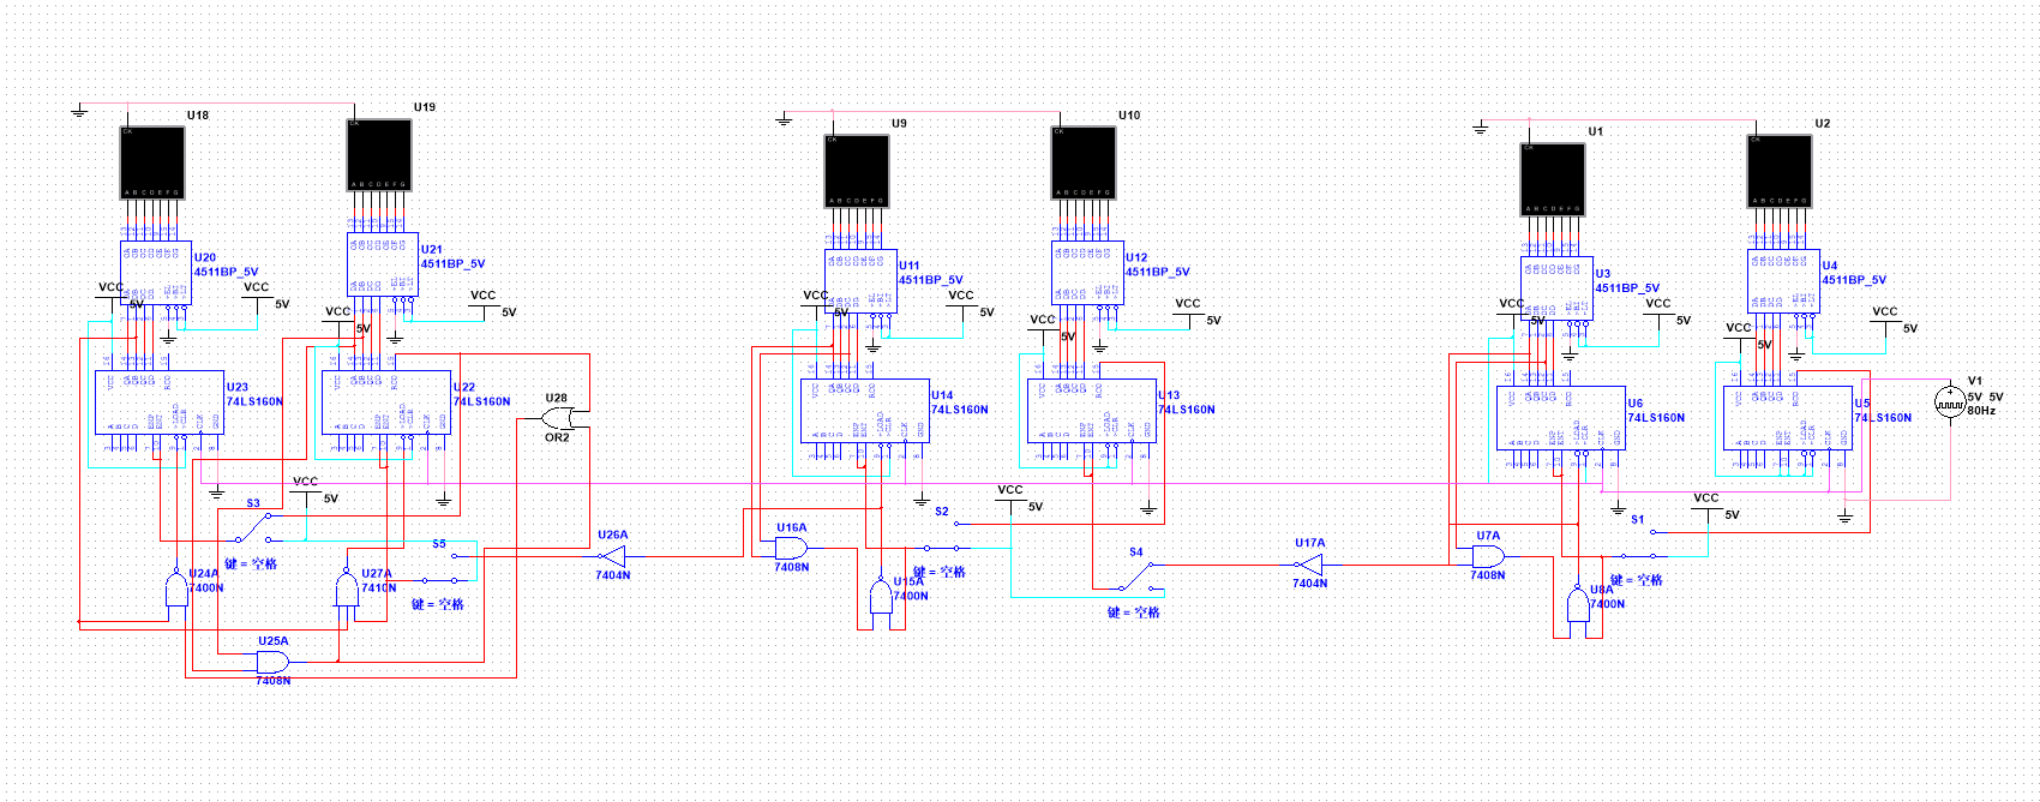
\includegraphics[width=0.9\textwidth]{2p2.png}
      \caption{74LS160仿真}
      \label{2p2}
    \end{figure}
    
  \subsection{数码显示模块}
  
  \subsubsection{数码显示模块数码管}
    
  电子时钟的显示电路主要由6个共阴极数码管，数码管译码器组成。其功能为可以显示电子时钟的示数，。
  我选择了共阴极数码管，所以选择74LS48作为数码管译码器。74LS48芯片是一种常用的七段数码管译码器驱动器，常用在各种数字电路的显示系统中，它可以可将BCD输入数据转换为七段显示器所需的控制信号。
  
  输出端（Ya－Yg）为高电平有效，可驱动灯缓冲器或共阴极VLED。当要求输出0-15时，消隐输入（BI）应为高电平或开路，对于输出为0 时还要求脉冲消隐输入（RBI）为高电平或者开路。当BI为低电平时，不管其它输入端状态如何，Ya－Yg均为低电平。当RBI 和地址端（A0－A3）均为低电平，并且灯测试输入端（LT）为高电平时，Ya－Yg为低电平，脉冲消隐输出（RBO）也变为低电平。当BI为高电平或开路时，LT为低电平可使Ya－Yg均为高电平。
  
  译码电路的功能是将“秒”、“分”、“时”计数器的输出代码进行翻译，变成相应的数字。用于驱动LED七段数码管的译码器常用的有74LS48。74LS48是BCD-7段译码器/驱动器，其输出是OC门输出且低电平有效，专用于驱动LED七段共阴极显示数码管。由74LS48和LED七段共阴数码管组成的一位数码显示电路如图所示。若将“秒”、“分”、“时”计数器的每位输出分别接到相应七段译码器的输入端，通过74ls48编码后再接到相应的数码管引脚上，便可进行不同数字的显示。
  

  \begin{figure}[H]
    \centering  %图片全局居中
    \subfigure[数码管仿真图片]{
    \label{1p1}
    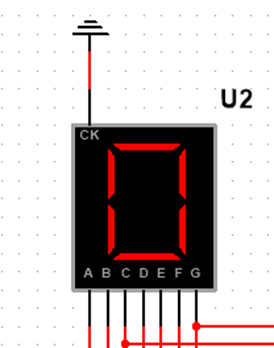
\includegraphics[width=0.35\textwidth]{1p1.png}}\subfigure[数码管引脚图]{
    \label{1p2}
    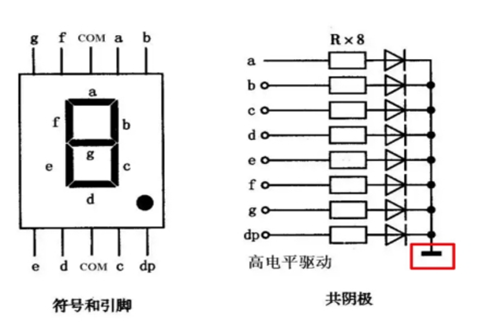
\includegraphics[width=0.63\textwidth]{1p2.png}}
    \caption{数码管}
    \label{555}
  \end{figure}
    
  \subsubsection{数码管显示}
  
  BCD-7段译码器/驱动器，其输出是OC门输出且低电平有效，专用于驱动LED七段共阴显示数码管。由74LS48和LED七段共阴数码管组成的一位数码显示电路如图所示。若将“秒”、“分”、“时”计数器的每位输出分别接到相应七段译码器的输入端，通过74ls48编码后再接到相应的数码管引脚上，便可进行不同数字的显示。

  在本实验中，我们使用了 4511BP 七段译码驱动器 来完成数字时钟的显示功能。
    4511BP 是一种功能强大的 CMOS BCD（Binary-Coded Decimal）到七段数码管的译码驱动芯片，
    能够将四位二进制编码信号转换为七段数码管的控制信号，实现直观的数字显示。
    它广泛应用于需要数字显示的场景中，例如计数器、计时器等。本芯片采用 16 脚双列直插封装（DIP-16），便于在面包板上使用，其低功耗和高稳定性特点使其非常适合数字电路实验。

    在输出端，4511BP 可以直接驱动共阳极七段数码管，而无需额外的电流放大器件。这简化了硬件设计，同时减少了功耗。在实验中，我们将计数器模块（74LS160N）的 BCD 输出连接到 4511BP 的 A、B、C、D 输入端，译码后驱动七段数码管，清晰显示秒、分、小时的计数值。
  
\begin{figure}[H]
  \centering  %图片全局居中
    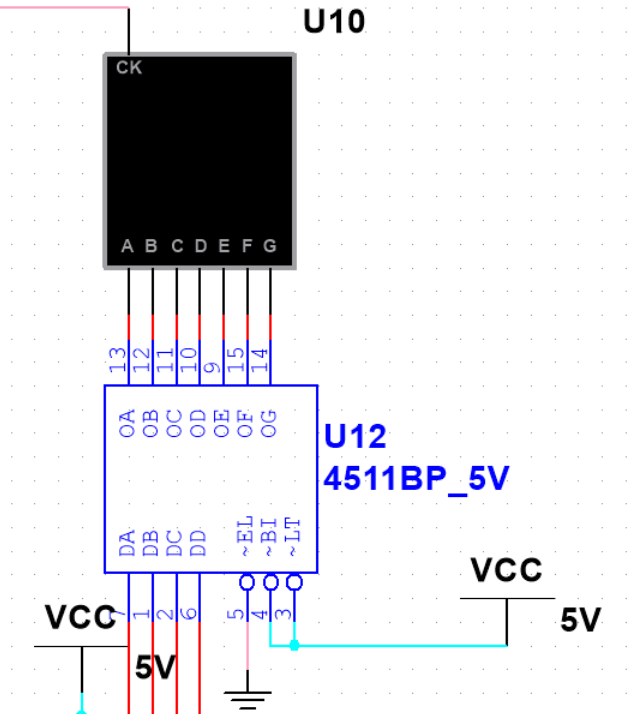
\includegraphics[width=0.5\textwidth]{xianshi}
    \caption{驱动器}
    \label{xianshi}
\end{figure}

\subsection{时钟模块}

\noindent\heiti{(1) 74LS160和74LS161选择}

\songti

\heiti{74LS160N}\songti 是一种可预置的同步十进制计数器，其计数范围为 0~9（十进制），当计数到 9 时自动清零，并生成进位信号（Ripple Carry Output，RCO）。它支持同步清零和
同步加载功能
 
    74LS160N的输入端包括四个
    数据输入端（D0~D3）、两个使能端（ENT、ENP）、一个清零端（CLR）和一个时钟端（CL
    K）。当使能端为高电平时，数据输入端的数据有效，计数器开始计数；当清零端为低电平时，计
    器清零；当时钟端接收到上升沿时，计数器进行计数。
 
    计数范围固定为 0~9，适合十进制计数应用（如秒、分钟计数）。
    提供同步清零和预置功能，易于初始化或调整计数值。
    输出自动复位到 0，简化进位逻辑设计。

74LS161 是一种可预置的同步四位二进制计数器，其计数范围为 0~15（二进制），当计数到 15 时自动清零，并生成进位信号（Ripple Carry Output，RCO）。它支持同步清零和
同步加载功能。

74LS161 的输入端包括四个
    数据输入端（D0~D3）、两个使能端（ENT、ENP）、一个清零端（CLR）和一个时钟端（CL
    K）。当使能端为高电平时，数据输入端的数据有效，计数器开始计数；当清零端为低电平时，计
    器清零；当时钟端接收到上升沿时，计数器进行计数。

    计数范围固定为 0~15，适合二进制计数应用（如秒、分钟计数）。
    提供同步清零和预置功能，易于初始化或调整计数值。
    输出自动复位到 0，简化进位逻辑设计。
在本次实验中，我初步使用了 74LS161，但在设计和调试小时计数器时，遇到了较大的复杂性问题，最终选择了更灵活的 74LS160 作为计数器核心。通过这一过程，我不仅加深了对两种计数器的理解，也学会了如何根据具体需求选择合适的器件和优化电路设计。
  74LS160 十进位特性，使其成为本实验数字时钟设计的最佳选择
  \begin{figure}[H]
    \centering  %图片全局居中
      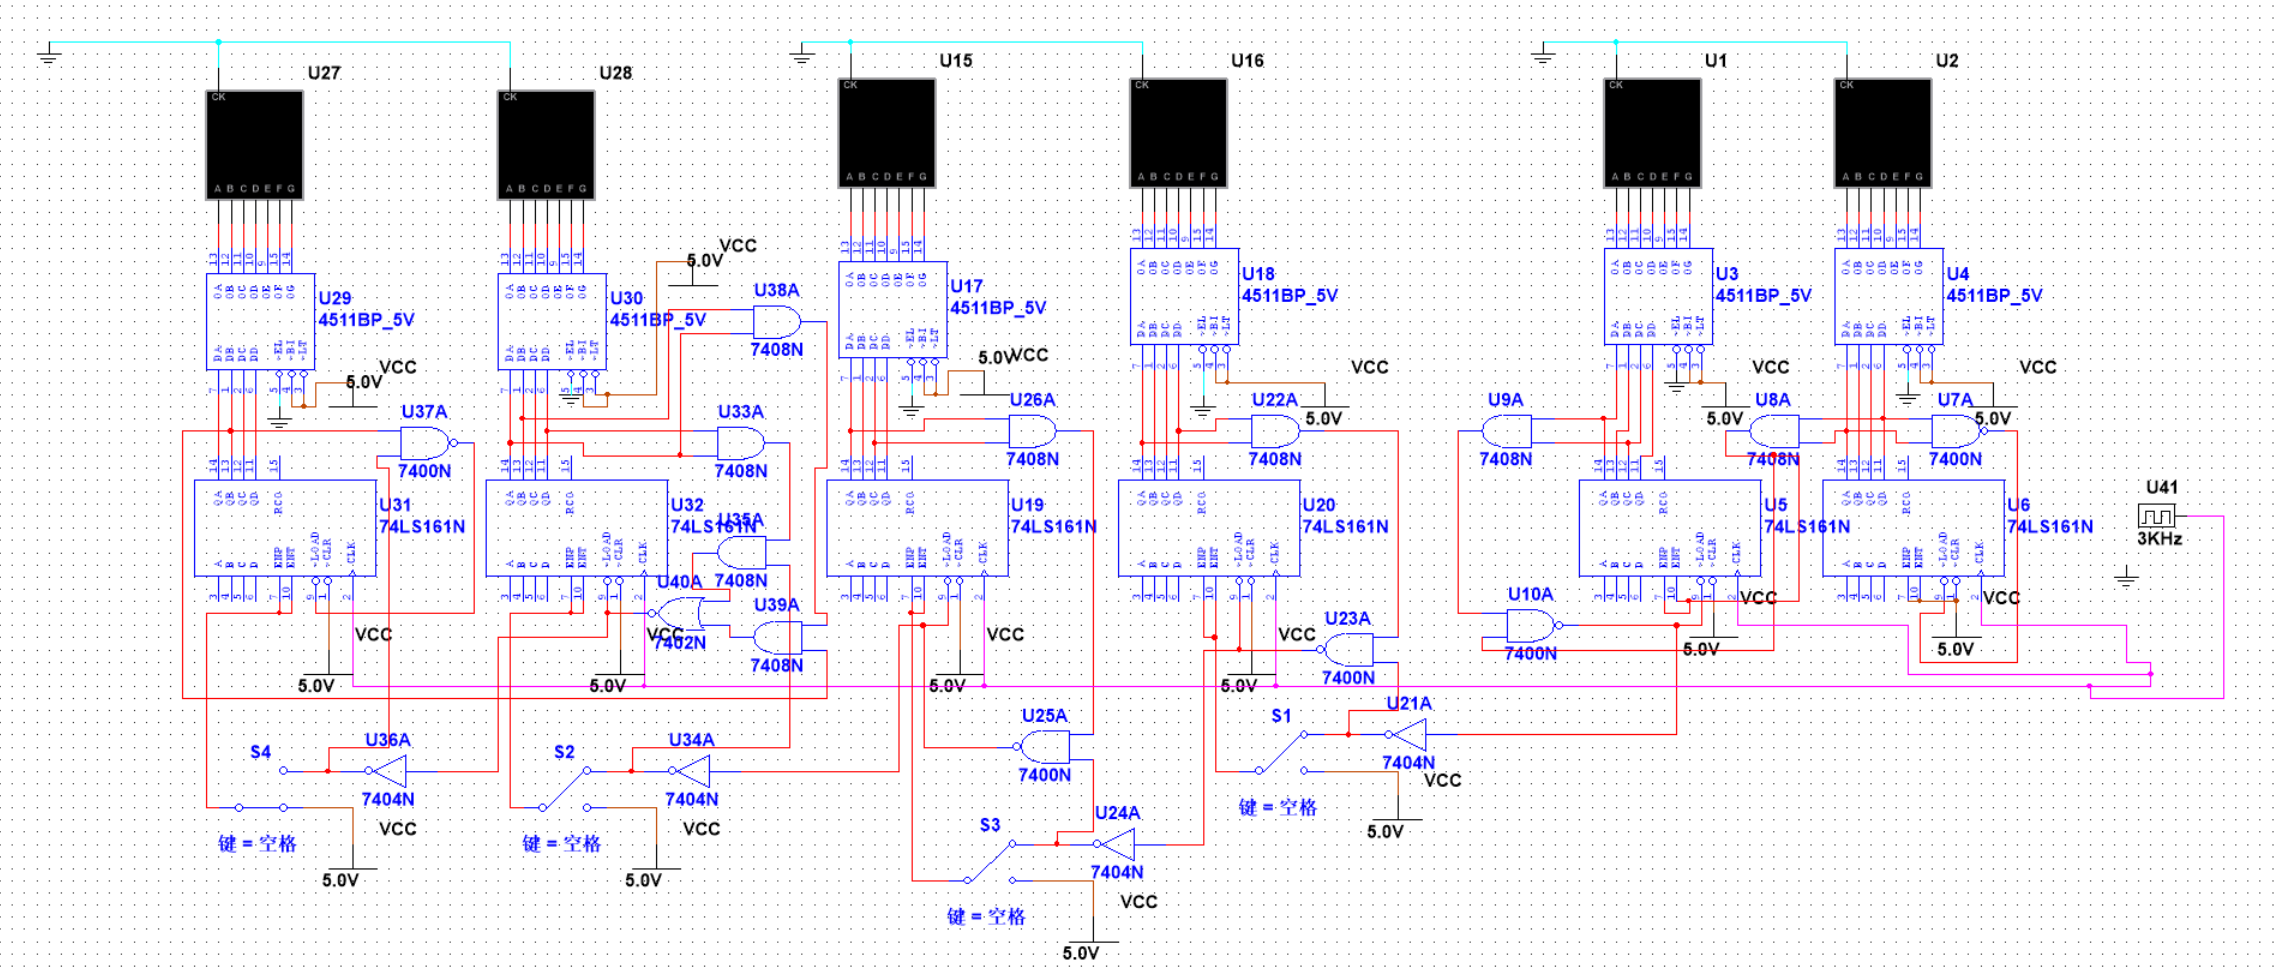
\includegraphics[width=0.9\textwidth]{2p1.png}
      \caption{74LS161仿真}
      \label{2p1}
    \end{figure}
    \begin{figure}[H]
      \centering  %图片全局居中
        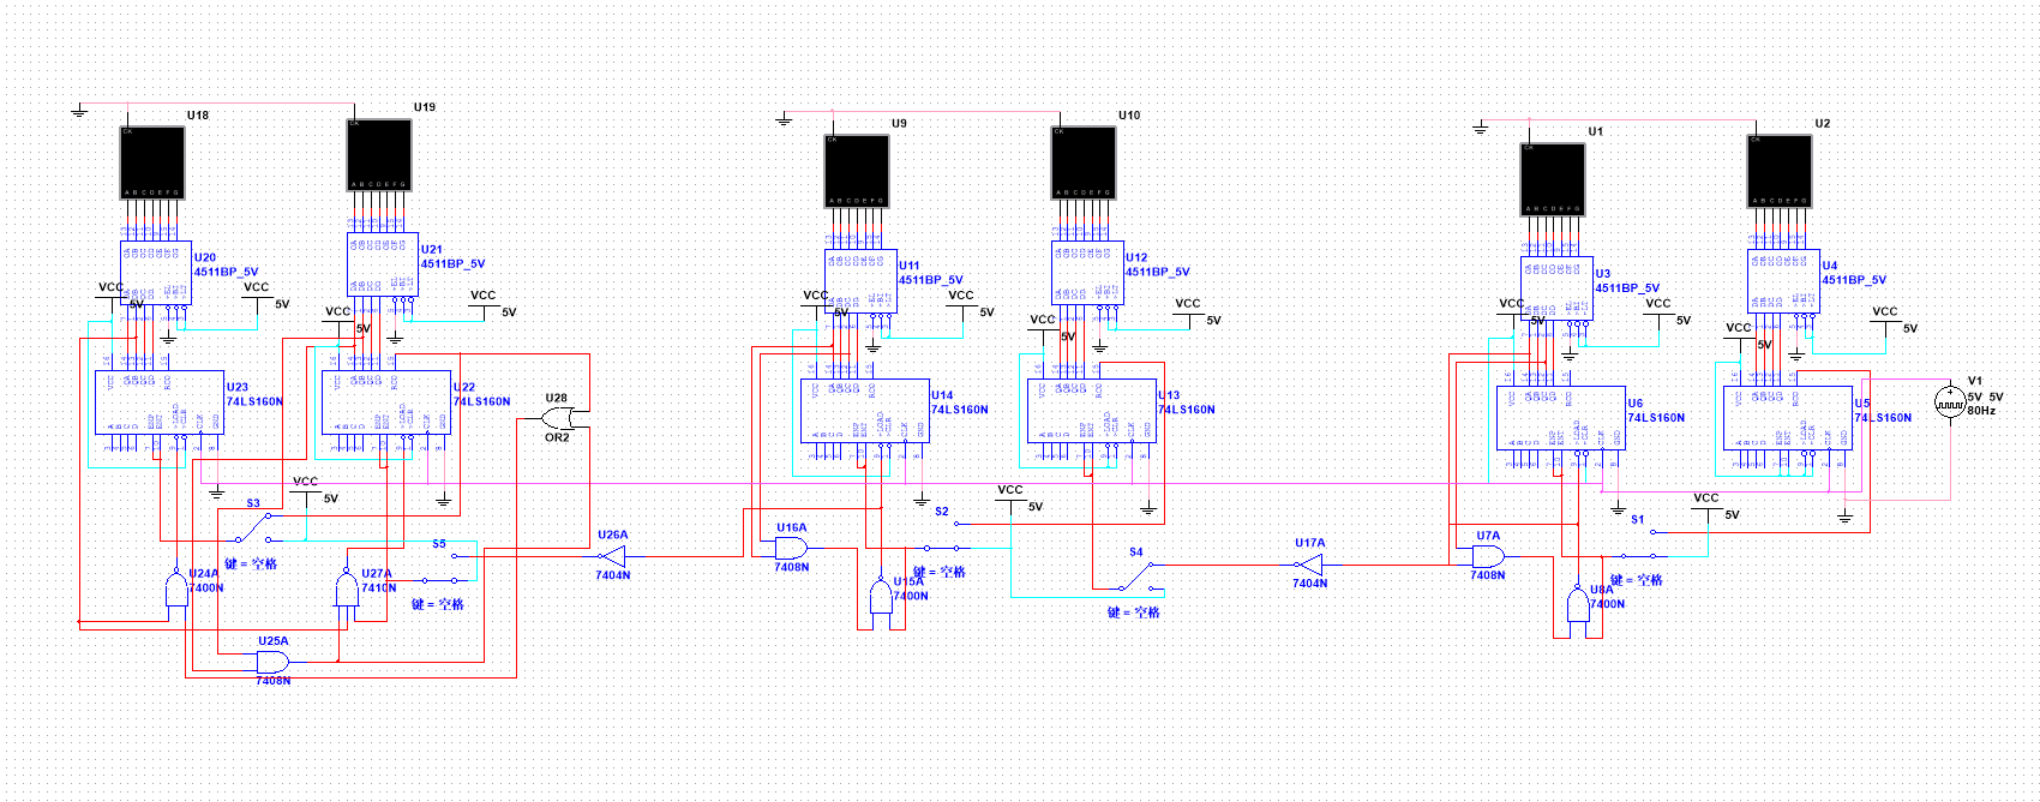
\includegraphics[width=0.9\textwidth]{2p2.png}
        \caption{74LS160仿真}
        \label{2p2}
      \end{figure}
      
 
      \noindent\heiti{(2)电路设计}


\songti
在本次数字时钟设计中，我采用了 74LS160 作为计数器的核心元件，并通过将每一级计数器的 CO（Carry Out） 输出口连接到上一位计数器的 EN（Enable） 使能输入口的逻辑设计，实现了各计数模块的联动工作。

具体来说，当当前位计数器达到最大计数值（如秒的个位达到 9）时，CO 输出一个高电平脉冲，触发上一位计数器（如秒的十位）开始计数，从而实现进位信号的传递。
这种设计方式充分利用了 74LS160 的内部进位信号功能，避免了额外的逻辑门电路来实现计数级联，从而使整个电路更加简洁清晰。

以秒计数器为例，个位计数器通过 CO 输出信号 驱动十位计数器，十位计数器在计数到最大值（5）时，再通过其 CO 输出 驱动分钟计数器。依此类推，实现了完整的秒、分钟、小时计数逻辑。

然而，这种设计也有一定局限性。例如，当用于小时高位（0~2）的计数时，74LS160 默认的十进制计数功能需要额外的逻辑约束以清零计数器，这增加了一定的设计复杂性。但总体而言，通过 CO 与 EN 的逻辑级联，大大简化了多级计数器的实现，提升了设计的可操作性和模块化程度。
\begin{figure}[H]
  \centering  %图片全局居中
    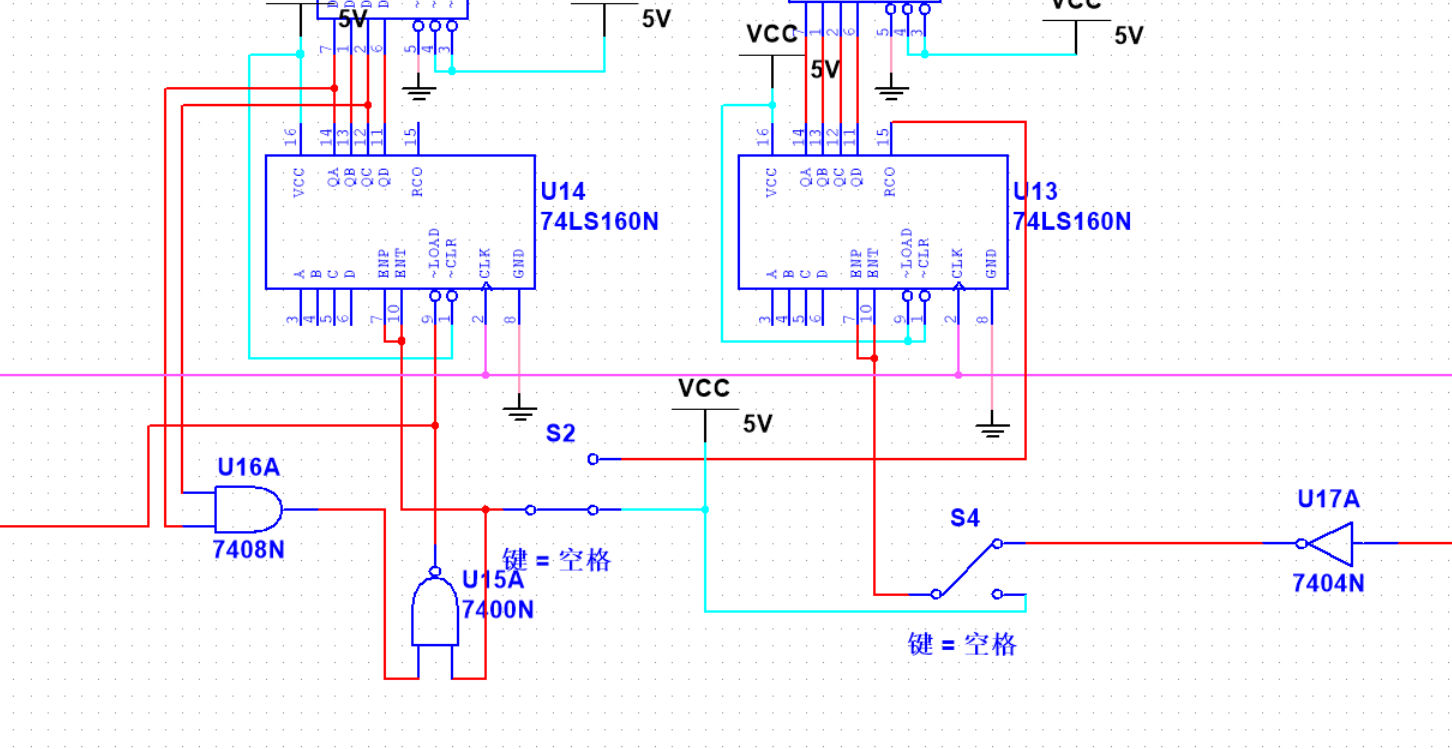
\includegraphics[width=0.75\textwidth]{luoji.png}
    \caption{时钟逻辑图}
    \label{luoji}
  \end{figure}

 24进制时计数器也是采用两片74ls160连接而成的。
  其低位也是十进制计数器，信号端接的是分单元的进位信号。
  高位的脉冲信号是时单元低位的进位信号。当高位计数为0001，低位为0010时，
  即时计数器计数到24时通过CLR清零端控制把时单元两片74ls160计数清零成00，这样就形成了24进制时计数器。其具体在电路中的接法如图所示。




\subsection{校时模块}


为了保证电路的稳定性和可靠性，我设计了一个校时电路，用于手动复位时钟计数器。校时电路由一个手动开关按键和一个与非门构成，当按键按下时，与非门输出低电平信号，清零所有计数器，实现时钟的复位功能。这样，即使在计数器工作过程中出现异常，也可以通过手动复位恢复正常工作状态。
  \begin{figure}[H]
    \centering  %图片全局居中
      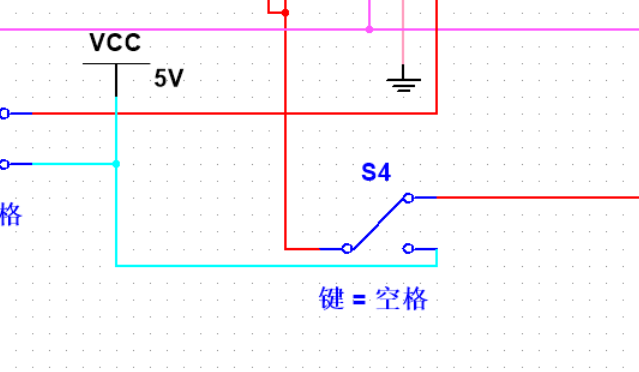
\includegraphics[width=1\textwidth]{fuwei.png}
      \caption{复位电路}
      \label{fuwei}
    \end{figure}




  \section{实验总结与收获}


\heiti{计数器级联逻辑设计}：\songti 我使用了 74LS160 的 CO（进位输出）接口作为下一位计数器的 EN（使能输入）信号，从而实现了各模块之间的联动计数逻辑。这种设计方式简洁高效，尤其是在秒与分钟的计数设计中，能够直接利用芯片内置的十进制计数功能，减少了额外的逻辑电路设计。

    然而，在设计小时模块时，由于小时高位（0~2）的计数需求不符合十进制逻辑，这部分需要通过逻辑门电路对 CO 信号进行约束，进一步对电路设计能力提出了挑战。在这一过程中，我学会了如何分析问题并优化设计，明确了不同计数器的适用场景。

    \heiti{不同计数器的对比} :\songti 在实验中，我分别尝试了 74LS160 和 74LS161 两种计数器芯片。通过实验发现：
    \begin{itemize}
      \item \heiti{74LS160} \songti 适合应用在计数范围固定为十进制的场景，其内置的十进制计数逻辑降低了秒和分钟计数设计的复杂性。
      \item \heiti{74LS161} \songti 由于其计数范围灵活，可通过逻辑约束实现非十进制计数（如小时高位 0~2），在复杂的数字时钟设计中具有更高的适应性。
      \item 通过对两种计数器的对比，我更加深入地理解了不同计数器的特性和适用场景，提升了对数字电路设计的认识。
    \end{itemize}
  
\heiti{调试与问题解决}：\songti 在本次数字时钟设计与实现的过程中，调试是非常重要的一环。实验中遇到了多个问题，我通过分析和调整，逐一解决了这些问题，也积累了宝贵的经验。以下是调试中遇到的主要问题以及对应的解决方案。
    \begin{itemize}
      \item \heiti{数码管闪烁} \songti 通过检查电路连接和信号波形，发现是接触不良导致的，通过重新连接电路解决了问题。
      \item \heiti{计数器无法清零} \songti 通过检查清零信号和使能信号，发现是逻辑门电路设计错误，通过修改逻辑电路解决了问题。
      \item 7400N和7401N的使用错误，导致了电路无法正常工作，通过查阅资料，重新设计电路解决了问题，发现同样是与非门，但是输入端的连接方式不同，导致了电路无法正常工作。
      \item 7400N和7401N的使用错误,后续实验中会优先分辨两种期间的使用。
    \end{itemize}
  \section{实验感悟}

本次实验让我深入理解了计数器芯片的工作原理和应用技巧。通过对比 74LS160 和 74LS161 的优缺点，我明白了根据具体需求选择元件的重要性。同时，在设计与调试的过程中，我也培养了分析问题、优化电路的能力。

此外，这次实验让我感受到电路设计中细节的重要性。比如在布线时，信号的走向、延时的影响以及电源的稳定性都会对电路整体运行产生显著影响。在未来的实验中，我将更加注重设计的系统性和调试的科学性，以进一步提升自己的设计水平

通过这次数字时钟的设计与实现，我不仅掌握了计数器级联设计的方法，还学会了如何解决实验中的实际问题。这次实验让我对数字电路的设计原则、调试技巧和逻辑优化有了全面的认识，也为后续更加复杂的数字电路设计打下了坚实的基础。



\end{spacing}
\end{document}


 % \section{实验过程}
  % \subsection{扫帚的选择}
  % 不同的扫帚参数各异，这里列出了部分扫帚的参数，请见表 \ref{broomsticks}。

  % % Insert a three-line table
  % \begin{table}[htbp]
  %   \centering
  %   \begin{tabular}{cccc}
  %     \toprule
  %     序号 & 名称 & 上市时间 & 最高时速 \\
  %     \midrule
  %     1 & 彗星290 & 1995年 & 60\,mph \\
  %     2 & 光轮1000 & 1967年 & 100\,mph \\
  %     3 & 光轮2001 & 1992年 & >\,100\,mph \\
  %     4 & 火弩箭 & 1993年 & 150\,mph \\
  %     \bottomrule
  %   \end{tabular}
  %   \caption{部分扫帚的参数对比}
  %   \label{broomsticks}
  % \end{table}


  % Insert source code
  % \lstinputlisting[style=cpp-style]{random.cpp}

  % Insert an image in a separate landscape page
  % \begin{landscape}
  %   \begin{figure}
  %     \centering
  %     
\includegraphics[width=\linewidth]{Nimbus2001}
  %     \caption{光轮2001扫帚}
  %     \label{Nimbus2001}
  %   \end{figure}
  % \end{landscape}

  % \begin{figure}
  %   % \centering
  %   
\includegraphics[width=\linewidth]{Nimbus2001}
  %   \caption{光轮2001扫帚}
  %   \label{Nimbus2001}
  % \end{figure}

  % \subsection{扫帚起竖}
  % 光轮 2001 扫帚如图 \ref{Nimbus2001} 所示，与麻瓜使用的扫帚相比，有以下区别：
  % \begin{enumerate}
  %   \item 扫帚末端较尖，同时在各个方向上都不是平面；
  %   \item 扫帚柄有一定弯曲，重心不易估计。
  % \end{enumerate}